The general idea for automatically finding the pervasive code patterns within a list of programs is to parse the programs and encode the important parts of the derived AST in fixed-size datapoints. We need fixed-size datapoints, as it is a requirement for both centroid-based and density-based well-known clustering algorithms. Work in this vein makes the assumption that each cluster corresponds to one change pattern.

Our pipeline for finding pervasive patterns in Rust programs also follows this idea. We decided to implement our pipeline completely in Python. To make this work, we need a way to get an AST as a Python dictionary. Syn \footnote{\url{https://crates.io/crates/syn}} is a Rust crate which is designed to be employed in Rust procedural macros. However, it includes a parser which is suitable for our purposes; we simply had to write a preprocessor to transform Syn AST output into Python dictionaries.

% TODO Define change
A change pattern categorizes a class of changes. We thus need to define what a change is. For our purposes, a change is ....
To compute the contents of a change, we need two code revisions: the revision before the commit, and the revision after it. After parsing these two revisions, we will have two ASTs, encoded in two Python dictionaries. A tree diff algorithm would specify the differences between two arbitrary trees. If the trees are abstracts syntax trees of programs, we simply call it an ASTDiff. We use dictdiff to obtain ASTDiffs.

An ASTDiff may include an arbitrary number of semantic changes. We are interested in finding the most important change within an ASTDiff and encoding that change in our datapoints. Sections \ref{sec:path_extraction} and \ref{sec:weighting_scheme} provide a detailed explanation of how we select the most important semantic information, which then helped us to obtain clusters that contained similar datapoints. 

We used Pydriller, which is a repository miner for Python. Our target repositories were the top 18 most starred open source Rust projects on GitHub. We mined all the bug related commits and ran them through our pipeline. Then, we applied the DBSCAN clustering algorithm on the obtained datapoints. In Section \ref{sec:clustering_data} we discuss why we chose DBSCAN for clustering and how we tuned it to improve clusters quality. 

\subsection{\label{sec:data_modelling}Data modelling}

\subsubsection{\label{sec:parsing_programs}Parsing Programs}

As mentioned above, we use Syn for parsing Rust. Syn handles all of Rust. Syn's nonterminals are primarily divided and implemented through two groups: Structs and Enums, which can be found on Syn webpage. The union of the item described in these two groups constitutes the list of our non terminals (\verb+NT+). The dimensions of our datapoints have been partly designed in a way that they adhere to the elements of \verb+NT+. The other part of our dimenstions is comprised of BC-related lexemes (\verb+BCL+), e.g. clone, Rc, Box, etc. The full list of \verb+BCL+ elements can be found within our artifact. We define dimension items as \verb+DI = NT+ $\cup$ \verb+BCL+, as this set also equals the columns of our tables.

We parse two versions of a Rust changed file in a commit; the file before the commit and after it. We will obtain two trees created by Syn. The change that transforms the first tree to the second one yields the fix which was applied in the commit. To find this difference, we use dictdiff, a Python library to find the diff of two Python dictionaries. Using the PLY tool (a Python implementation of lex and yacc), we wrote a simple transformer from the Rust AST into Python dictionaries. After obtaining the syntax trees in Python dictionary format, we can use dictdiff to determine the ASTDiff. 

dictdiff tool provides modifications' types: 
\begin{itemize}
\item `add': A new structure has been added to the tree; 
\item `remove': A structure has been dropped from the tree; 
\item `change': The content of a sub structure of the first tree has changed.
\end{itemize}
dictdiff also determines the context within which the modification has occured. This context happens to be the root elements in our file, e.g. function blocks, struct blocks, impl blocks, etc. The modified content within a context is still in the form of tree. Our objective right now is to find primary elements in our diff that describe the semantics of occurred change.
% TODO rework the above paragraph

\subsubsection{\label{sec:path_extraction}Path Extraction}

\begin{figure}[h]
\centering
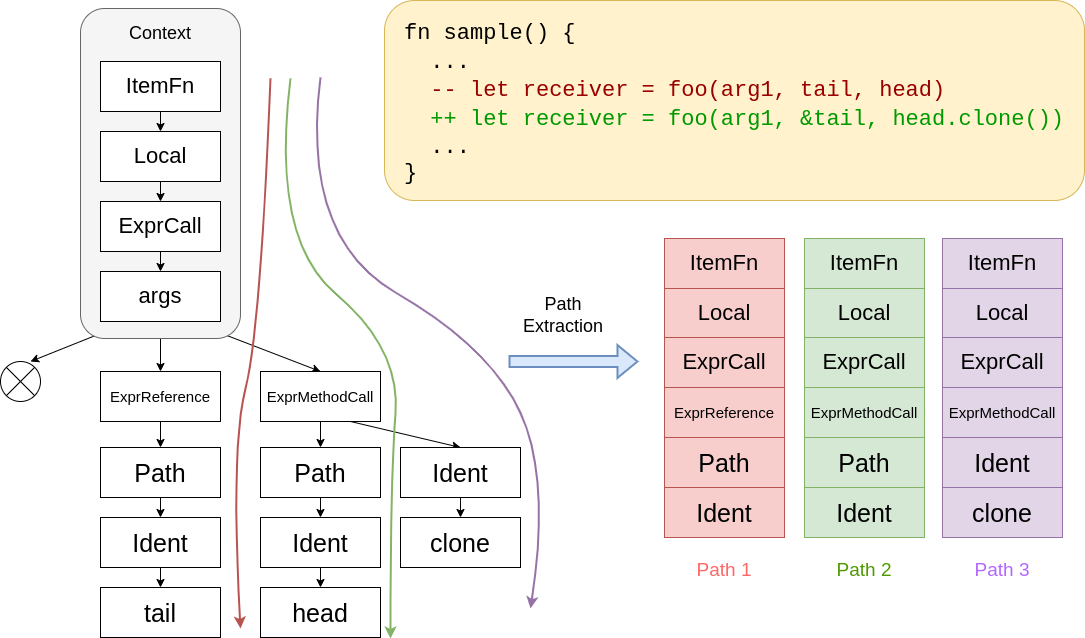
\includegraphics[width=0.8\textwidth]{figs/extraction.png}
\caption{\label{fig:extraction}Path Extraction}
\end{figure}

The output of dictdiff is a list of diffs, where each diff comprises three parts. The first part specifies whether the modification is of type 'add', 'remove', 'change'. The second part identifies the context of the modification, that is, the path from the root of the tree to the subtree in which the modification has occured. The third part is the content of the change (terminals and nonterminals). Our tool looks for changes within each root-level scope. That is, our assumption is that a change pattern occurs within one root-level scope. In this work, we chose to not handle patterns that involve changes in multiple functions or multiple files. However, our tool would detect both continuous and non-continuous line changes within one scope.
% TODO provide an example and then transform it into fig:extraction. 

Looking at the tree encoded in the content part of each diff, we realized that each path to a leaf represents one contributing element to the change. Through a Depth First Search we can collect all of these paths. We store only the nodes that exist in the \verb+DI+. The outcome of the DFS search is a set of paths.

Figure~\ref{fig:extraction} shows a simple change and its respective paths. The change replaces \verb+tail+ with \verb+&tail+ and \verb+head+ with \verb+head.clone()+. That is, after the change, the second argument passes a borrow of \verb+tail+ rather than sending the ownership of \verb+tail+ to the callee; and, in the third argument, instead of sending \verb+head+ to the callee, it sends a clone of it. A DFS search on this tree would yield three different paths, which we show in red, green, and purple. The path represents the sequence of involved non terminals, which represents one contributing factor to the change. We found it crucial to record the order of all path nodes as it gives us freedom to control the order-sensitiveness in our datapoint encoding.

The next question is how to transform these paths to a fixed size datapoint. First, we need to define a fixed set of columns. The number of columns would depend on the amount of information we want to encode in the datapoints. The most naive approach would be to only report the observed non terminals within the diff. That yields a fully order-insensitive representation. In such an encoding, for instance, there is no difference between two nested if statements and two if statements beside each other. Theoretically, to reach full order-sensitiveness, we would need encode all possible combinations of dimension items as our dimensions, which yields a large number (A loose upper bound would be $n^n$ where $n$ is the number of dimension items). Apart from that, not all combinations adhere to Rust syntax. A reasonable work around would be to reduce from the full set of nonterminals to a smaller set of categories (e.g. A category for larger entites like class or function definitions, and a category for smaller entities like statements and expressions), and then to set the dimension as all possible combinations of these categories (Similar to JS paper, ref). This would reduce the number of dimensions and provide more reasonable and syntactically-correct combinations. However, this would still yield a sparse dataset. 

In our methodology, we propose a novel method. Similar to the first approach, we define the columns of our dataset, as the set of dimension items we collected from Syn. However, to achieve an acceptable level of order-sensitiveness, we carried out two auxiliary steps. First, we record the number of occurrences of dimension items within the paths at each scope. The reason behind this decision is because a different order of program elements yields a different number of occurrences of underlying dimension items. Second, we semi-automatically design a weighting scheme to prioritize non terminals that we think are more salient for Rust bugs.

\subsubsection{\label{sec:weighting_scheme}Weighting Scheme}

Our main objective is that our datapoints manifest the change with high level of precision. For instance, the purple (right-most) path in Figure~\ref{fig:extraction} could be described as a change in a local variable declaration; a change in a function call; calling a method of one of the function arguments; or calling clone() on one of the function arguments. The last description offers the most accurate description. The whole idea behind our weighting scheme is to be able to identify the change accurately. 

% I need to reread this key paragraph. - PL
A simple heuristic is that, the closer we get to the leaves in the ASTDiff, the more important dimension items get. Another observation is that the elements closer to the root tend to be repeated in all the paths within one ASTDiff (e.g. ItemFn, Local, ExprCall in Figure~\ref{fig:extraction}). Exploiting the latter observation, to obtain a basic knowledge about the number of repetitions of dimension items, we mined the last 20 bug related commits of the last 20 most starred rust projects on GitHub, and ran them through of pipeline. We recorded the number of occurrences of each dimension item in total. Then we gave the value of the inverse of the number of occurrences to each token. The intuition is that the higher the number of occurrences of a dimension item, the closer it is usually seen to the root. Hence, it probably does not provide us with the most accurate description of the change. In addition to that, as we wanted to make sure that our tool captures the patterns related to borrow checker, we manually raised the weights of the dimension items related to borrow checker. That is why we characterize our weighting scheme as semi-automatically designed. 

\subsection{\label{sec:mining_repositories}Mining Repositories}

\begin{figure}[h]
\centering
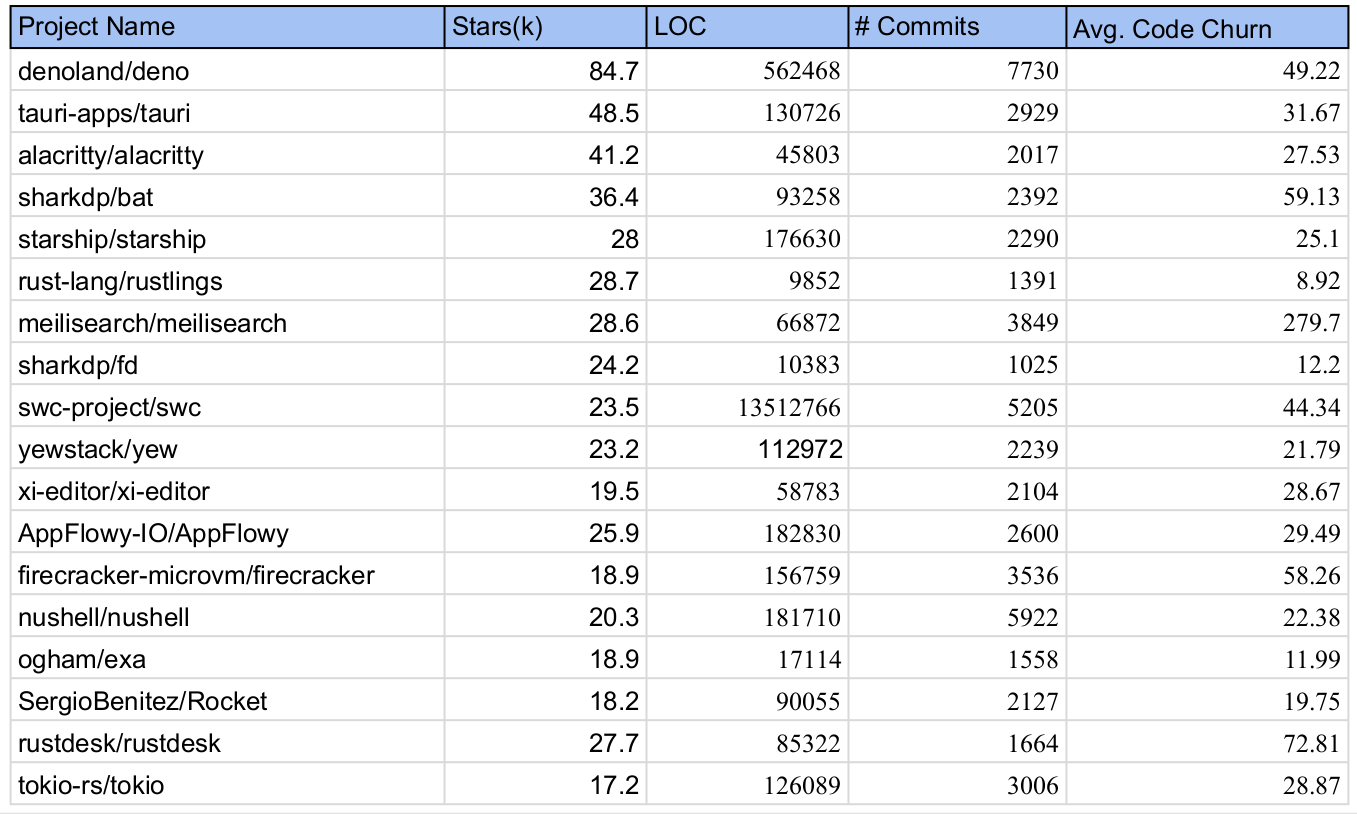
\includegraphics[width=1\textwidth]{figs/repos.png}
\caption{\label{table:repos} Target Repositories}
\end{figure}

Now that we have set up our code analysis pipeline, we can start mining the Rust repositories. We target the top 18 most starred Rust projects on GitHub, at the time of data collection. The details of these projects are outlined in Table \ref{table:repos}. We computed the average code churn of the files within the projects. denoland/deno and swc-project/swc are the projects with largest number of LOCs and average code churn. Unsurprisingly, we captured a lot of instances from these two projects in our final clusters.

We use Pydriller, a Python library for mining software repositories. Pydriller provides APIs to extract commits from a Git repository, and search through different revisions of files. Algorithm \ref{alg} shows how we leveraged Pydriller to run the target repositories through our code analysis pipeline, and populate two databases; one for general patterns and one for borrow-checker related patterns. The borrow-checker related patterns are the changes that include certain keywords (e.g. clone, Box, etc. Full list can be found in our artifact). For each repository, we search through all the commits that include bug fixing related keywords within their commit messages. These keyword for the scope of our project are `bug', `error', `fault', `defect', and `fix'. 

Next, we collect a pair of revision per each Rust file. The pair includes the state of the file before commit and after commit ($f_a, f_b$). After parsing each revision and computing the ASTDiff, we can obtain the fixed sized datapoint $DP$. If the datapoint contains borrow-checker related keywords, we would put that inside the BC-related code changes table ($D_b$), otherwise we would put it in the general code changes table ($D_g$). In both cases, we augment the datapoint with the commit hash, filename, and the scope in which the change has happened. In case of BC-related code changes, we also store detected BC-related keyword. Now our tables are ready for clustering and categorization.

\begin{algorithm}
\caption{\label{alg} Mining Algorithm}
\hspace*{2mm} \textbf{Input:} $R$ (target repositories)  \\
\hspace*{2mm} \textbf{Output:} $D_g$ (General code changes) \\
\hspace*{2mm} \textbf{Output:} $D_b$ (BC-related code changes)
\begin{algorithmic}
\State $D_g \leftarrow \phi$
\State $D_b \leftarrow \phi$
\For{$r \in R$}
    \For{$c \in \textsc{ExtractCommits}(r)$}
        \If{$c.msg$ contains bug fixing related keywords}
            \For{$\{f_b, f_a\} \in \textsc{GetModifiedRustFiles}(c)$}
                \For{$e \in \textsc{ASTDiff}(\textsc{Parse}(f_b), \textsc{Parse}(f_a))$}
                    \State $DP \leftarrow \textsc{GetDataPoint}(e)$
                    \State $DP \leftarrow c.hash \cup f_a.name \cup e.scope \cup DP $
                    \If{$\textsc{IsBCRelated}(e)$}
                        \State $DP \leftarrow \textsc{GetBCKeyword}(e) \cup DP $
                        \State $D_b \leftarrow D_b \cup DP$
                    \Else
                        \State $D_g \leftarrow D_g \cup DP$
                    \EndIf
                \EndFor
            \EndFor
        \EndIf
    \EndFor
\EndFor
\end{algorithmic}
\end{algorithm}

\subsection{\label{sec:clustering_data}Clustering Data}

We use DBSCAN clustering algorithm for two main reasons. Firstly, it is a density-based clustering method, which means that it detects arbitrarily shaped clusters as opposed to centroid-based methods, like k-means. Secondly, also in contrast to k-means, it does not require the number of clusters in advance as an input to the algorithm.

There are two parameters that need tuning in DBSCAN. First parameter is $\epsilon$ which indicates a radius with which you can decide whether a point is a core point, a border point, or an outlier. Second parameter is the minimum number of point you would like each cluster to have. We denote his parameter with $Z$. We ran DBSCAN using different combinations of these two parameters. In Figure \ref{fig:clustering}, we show nine different experiments with their respective parameter values. Within each subplot, the number of clustered points, noise points, and the number of clusters have been specified both for $D_g$ and $D_b$. 


\begin{figure}[h]
\centering
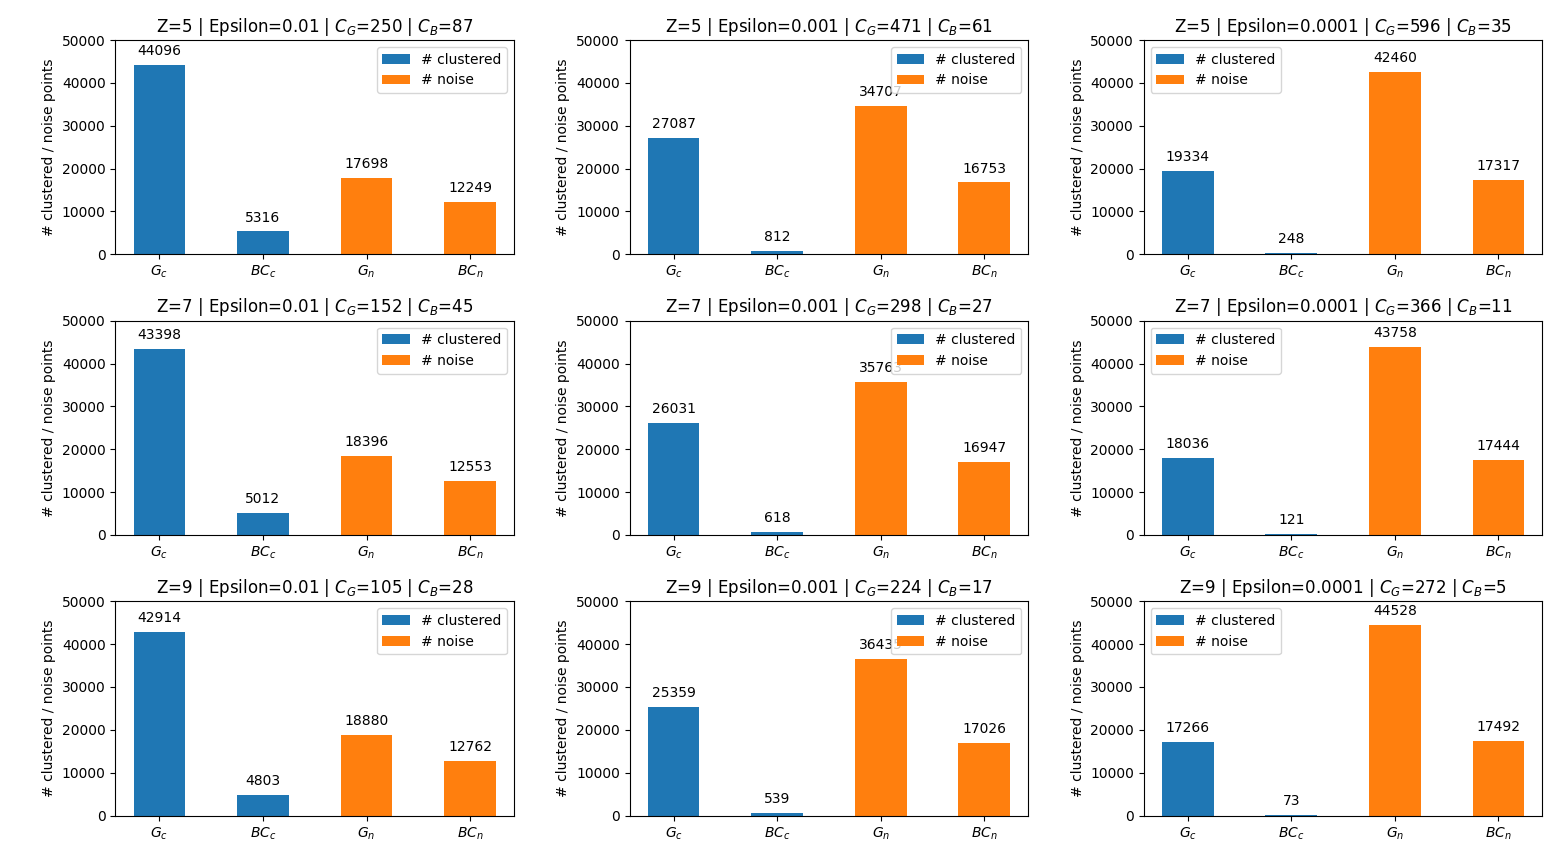
\includegraphics[width=1\textwidth]{figs/clusters.png}
\caption{\label{fig:clustering} Clustering Experiments}
\end{figure}

As a general rule, a lower value for $Z$ would allow more group of close points to be considered as clusters, resulting in a higher number of clusters. A large value for $\epsilon$ would widen the search radius, allowing more points to fall in the clusters which results in a reduction of the number of noise points. That possibly can put points that do not completely manifest same patterns inside a cluster, resulting in a ineffective clustering. Alternatively, a small value for $\epsilon$ would tighten the ring of search, possibly separating clusters which essentially manifest same code changes. Also if $\epsilon$ is really small, the clustering algorithm might not detect some clusters at all, resulting in a reduction of the number of clusters. 

\subsubsection{\label{sec:manual_analysis_parameter_tuning}Manual Analysis for parameter tuning}

That is why, we carried out a manual analysis of clusters. In the manual analysis we randomly pick 50 clusters and from each cluster we randomly choose 10 datapoints. The analyzer then looks at the code and specify the clusters that contained more than five datapoints showing similar patterns. Through the manual analysis we specified that $\epsilon=0.0001, Z=5$ and $\epsilon=0.001, Z=5$ acted as the best parameters for $D_g$ and $D_b$, resulting in 596 and 61 clusters, respectively. As the final step, we exclude the clusters that contained datapoints from less than 3 projects. That is because, we wanted our clusters to contain cross-project patterns as much as possible.  

\subsubsection{\label{sec:manual_analysis_cluster_selection}Manual Analysis for cluster selection}
% 3 types, refactoring dropped

Similar to ..., following Cotroneo et al. definitions, we divide the clusters in three different groups:

\begin{itemize}
    \item bug-fix: "The changed code actually fixes the behavior of software, which can represent fixes for a bug type". We consider the changes that improve program performance as instance of this group, as they fix the behavior of software.
    
    \item fix-induced: "The changed code is a group of bug-fixing code changes but not represents an actual bug fix, e.g., adding new input parameters to a method, the method signature and method call must be changed corresponding".
    
    \item refactoring: "the changed code does not modify the software behavior, e.g., better readability or encapsulation".
\end{itemize}

In this work, we were only interested in the first two group and disregarded the the clusters that manifest a refactoring change. Also, we prefer reporting clusters that manifest concrete patterns. An abstract pattern as opposed to a concrete pattern can account for many changes in the programs. For instance, the pattern `Adding a new statement to a function's body' is deemed more abstract than `Changing a clone of a variable to a borrowing of it in a function argument'.

In our manual analysis, we randomly picked 50 datapoints of each cluster. If the cluster had less than 50 datapoints, we would analyze all of the datapoints in the cluster. Next, we read the code and also the bug report related to all the datapoints (if existed). In case that a similar pattern was detected over the instances of a cluster, we would write a natural language description of that cluster. After providing all the descriptions, we linked similar clusters together as possible candidates for merging. At last, after accomplishing re-examination for merge possibilities, we selected 19 clusters that manifested concrete changes. We discuss about our findings in Section \ref{sec:common_patterns} and \ref{sec:bc_patterns}.




